% !TeX spellcheck = cs_CZ
{\tikzset{external/prefix={tikz/CES/}}
 \tikzset{external/figure name/.add={ch04_}{}}
%---------------------------------------------------------------------------------------------------
% file technology.tex
%---------------------------------------------------------------------------------------------------
%==============================Kapitola: Číslicové součástky a technologie=========================
\chapter{Číslicové součástky a technologie}
\minitoc

  \section{Rozdělení číslicových integrovaných obvodů}
    Logické integrované obvody zpracovávají nespojité signály, které nabývají jen konečného malého
    počtu úrovní. Naprostá většina dnes vyráběných logických IO využívá pouze dvou logických úrovní
    pracujících s dvojkovou číselnou soustavou. Jejich funkci a vzájemné spojování do soustav lze
    popsat pomocí Booleovy algebry (viz kap. \ref{CES:basic_bool_alg}) \cite[p.~8]{Musil2002}.
    
    Digitální IO se vyrábějí v technologii \emph{bipolární} (kap. \ref{CES:Bipolar_technology}) i
    \emph{unipolární} \ref{CES:Unipolar_technology} (především MOS). Základní kriteria, podle
    kterých posuzujeme kvalitu (vhodnost pro danou aplikaci) jednotlivých druhů (tříd) digitálních
    obvodů jsou:
    \begin{itemize}\addtolength{\itemsep}{-0.5\baselineskip}
      \item rychlost,
      \item příkon,
      \item odolnost proti rušení,
      \item široký rozsah pracovních teplot,
      \item nízké rušení generované vlastním obvodem (proudové špičky při změnách stavu),
      \item snadnost realizace složitějších logických funkcí,
      \item dosažitelná hodnota základních hradel a možnosti velké integrace,
      \item nízká cena.    
    \end{itemize}
    Tyto požadavky splňuje každá třída digitálních obvodů pouze částečně. Proto se ve výrobě
    udržuje několik různých tříd digitálních obvodů, z nichž každá má zdůrazněnou některou z výše
    uvedených vlastností tak, jak to odpovídá její fyzikální podstatě.
   
    \subsection{Vlastnosti logických hradel}
  
  \section{Bipolární digitální obvody}\label{CES:Bipolar_technology}
      V bipolární technologii jsou skupiny logických obvodů charakterizovány z hlediska režimu
      činnosti tranzistorů a tvoří dvě základní skupiny. Jsou to logické IO - s tranzistory
      pracujícími:
      \begin{itemize}
        \item v saturaci: tranzistor spínán z vypnutého stavu do saturace,
        \item v nesaturačním - aktivním režimu: tranzistor přepínán mezi stavem vypnutým (nebo
              slabě sepnutým) a aktivním (nesaturačním) módem.
      \end{itemize}
      V obou skupinách je přepínanou součástkou \emph{tranzistor NPN}. \emph{Komplementární
      tranzistor PNP} je využíván pouze jako zatěžovací prvek nebo jako proudový zdroj; pro tyto
      účely se rovněž využívá i rezistor.
      \begin{figure}[ht!]
        \centering
        \subfloat[Součtový člen]{\label{ces:fig_D_OR}
          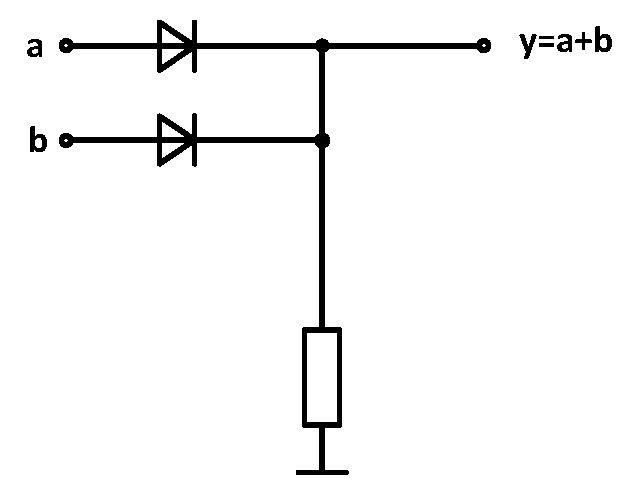
\includegraphics[width=0.3\linewidth]{diodovy_log_OR.pdf}}
        \subfloat[Součinový člen]{\label{ces:fig_D_AND}
          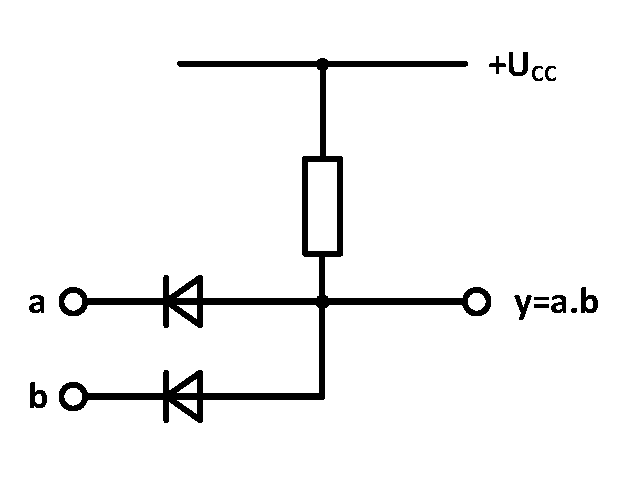
\includegraphics[width=0.3\linewidth]{diodovy_log_AND.pdf}}
        \caption{Diodová logika}
        \label{CES:fig_diodova_logika}
      \end{figure}
   \section{Unipolární digitální obvody}\label{CES:Unipolar_technology} 
  %-------------Přizpůsobení logických obvodů různých napěťových tříd-----------------------------
  % source: AN/Microchip/AN_3V_5V_Digital_Interfacing.pdf
  \newpage
  \section{Přizpůsobení logických obvodů různých napěťových tříd} %Digital Interfacing
    % When interfacing two devices that operate at different voltages, it is imperative to know the
    % output and input thresholds of both devices. Once these values are known, a technique can be
    % selected for interfacing the devices based on the other requirements of your application.
    % Table \ref{CES:tab_threshold} contains the output and input thresholds that will be used
    % throughout this document. When designing an interface, make sure to reference your
    % manufacturers data sheet for the actual threshold levels.
    Vyskytne-li se v číslicovém návrhu potřeba použít logická hradla z odlišných napěťových tříd,
    budeme postaveni před problém jejich vzájemného propojení zachovávající jejich funkčnost. Pro
    správnou volbu vhodného napěťového přizpůsobení logických hradel z různých rodin, je nutné znát
    nejen jejich rozhodovací napětí, ale také následující parametry, které jsou uvedeny v tabulce
    \ref{CES:tab_threshold} \cite[p.~22]{DS41285A}:
    
    \begin{itemize}\addtolength{\itemsep}{-0.5\baselineskip}
      \item maximální úroveň logické '0' na vstupu hradla - $\mathbf{V_{IL_{max}}}$
      \item minimální úroveň logické '1' na vstupu hradla - $\mathbf{V_{IH_{min}}}$
      \item maximální úroveň logické '0' na výstupu hradla - $\mathbf{V_{OL_{max}}}$
      \item minimální úroveň logické '1' na výstupu hradla - $\mathbf{V_{OH_{min}}}$
    \end{itemize}
    
    \begin{table*}
      \centering
      \begin{tabular}{|>{\columncolor{Tan}}l||c|c|c|c|}
        \hline
        \rowcolor{CornflowerBlue}{ }    & {$\mathbf{V_{OH_{min}}}$} & {$\mathbf{V_{OL_{max}}}$} & %
                                          {$\mathbf{V_{IH_{min}}}$} & {$\mathbf{V_{IL_{max}}}$} \\
        \hline
        \hline
        \texttt{5V TTL}                       
                    & 2.4V            & 0.5V       & 2.0V              & 0.8             \\
        \hline
        \texttt{3.3V LVTTL}          
                    & 2.4V            & 0.4V       & 2.0V              & 0.8             \\
        \hline
                    & 4.7V            & 0.5V       & 3.5V              & 1.5V            \\
        \multirow{-2}*{\texttt{5V CMOS}}      
                    & ($V_{CC}$-0.3V) &            & (0.7x$V_{CC}$)    & (0.3x$V_{CC}$)  \\
        \hline
                    
                    & 3.0V            & 0.5V       & 2.3V              & 1.0V            \\
        \multirow{-2}*{\texttt{3.3V LVCMOS}} 
                    & ($V_{CC}$-0.3V) &            & (0.7x$V_{CC}$)    & (0.3x$V_{CC}$)  \\
        \hline 
      \end{tabular}
      \caption{Rozhodovací úrovně napěťových tříd: \texttt{5V TTL}, \texttt{3.3V LVTTL}, 
                                                   \texttt{5V CMOS}, \texttt{3.3V
      LVCMOS}}\label{CES:tab_threshold}
    \end{table*}
    Úroveň logické nuly a jedničky na výstupu určuje konstrukce koncové části digitálního obvodu.
    Nejčastější provedení jsou na obr. \ref{ces:fig_digit_out_common}. Jsou-li různé digitální
    obvody připojeny na společnou sběrnici, může dojít k situaci, kdy některý z výstupních vývodů
    bude buzen vyšším napětím než je napájecí napětí příslušného obvodu. I v tomto případě výstupní
    část digitálního obvodu rozhoduje o výsledném chování. Shrňme základní vlastnosti technologií
    číslicových obvodů uvedených na obr. \ref{ces:fig_digit_out_common}:
    \begin{itemize}
      \item Bipolární koncový stupeň nedovoluje plný rozkmit výstupního signálu. Je-li obvod
            napájen \SI{5}{\volt}, je výstup při úrovni H limitován na $V_{CC}-2\times V_{BE}$(cca
            3.6V). To je hodnota, která na rozhraní \SI{3}{\volt} systému nezpůsobuje příliš velký
            napěťový rozdíl, a tedy proudu, tekoucímu z napájecího zdroje \SI{5}{\volt} systému do
            zdroje \SI{3}{\volt} systému.
      \item Výstupní napětí typické \texttt{CMOS} součástky se prakticky pohybuje v rozsahu
            \texttt{GND} - \texttt{VCC}.
      \item Některé součástky mají výstup typu \emph{open kolektor - OC} resp. \emph{open drain -
            OD}, tj. neexistuje vnitřní obvod, jenž by uvedl výstup do stavu H. K tomu je zapotřebí
            \emph{pull-up} rezistoru, který připojí výstup k napětí, které může být i vyšší než je
            napájecí - \texttt{VCC}. Očividně, tento způsob umožňuje relativně snadné rozhraní, ale
            pro dosažení vyšších rychlostí je nutné volit relativně malý odpor, což zvyšuje
            spotřebu.
      \item U \texttt{NMOS} stupně je podobně jako u bipolárního stupně výstupní napětí logické
            úrovně H omezeno úbytkem na kanálu horní NMOS tranzistoru na $V_{CC} - V_{TH}\simeq
            \SI{3.5}{\volt}$. Obvykle je tedy možné přímé řízení 3V systému.
    \end{itemize}

    \begin{figure}[ht!]
         \centering
         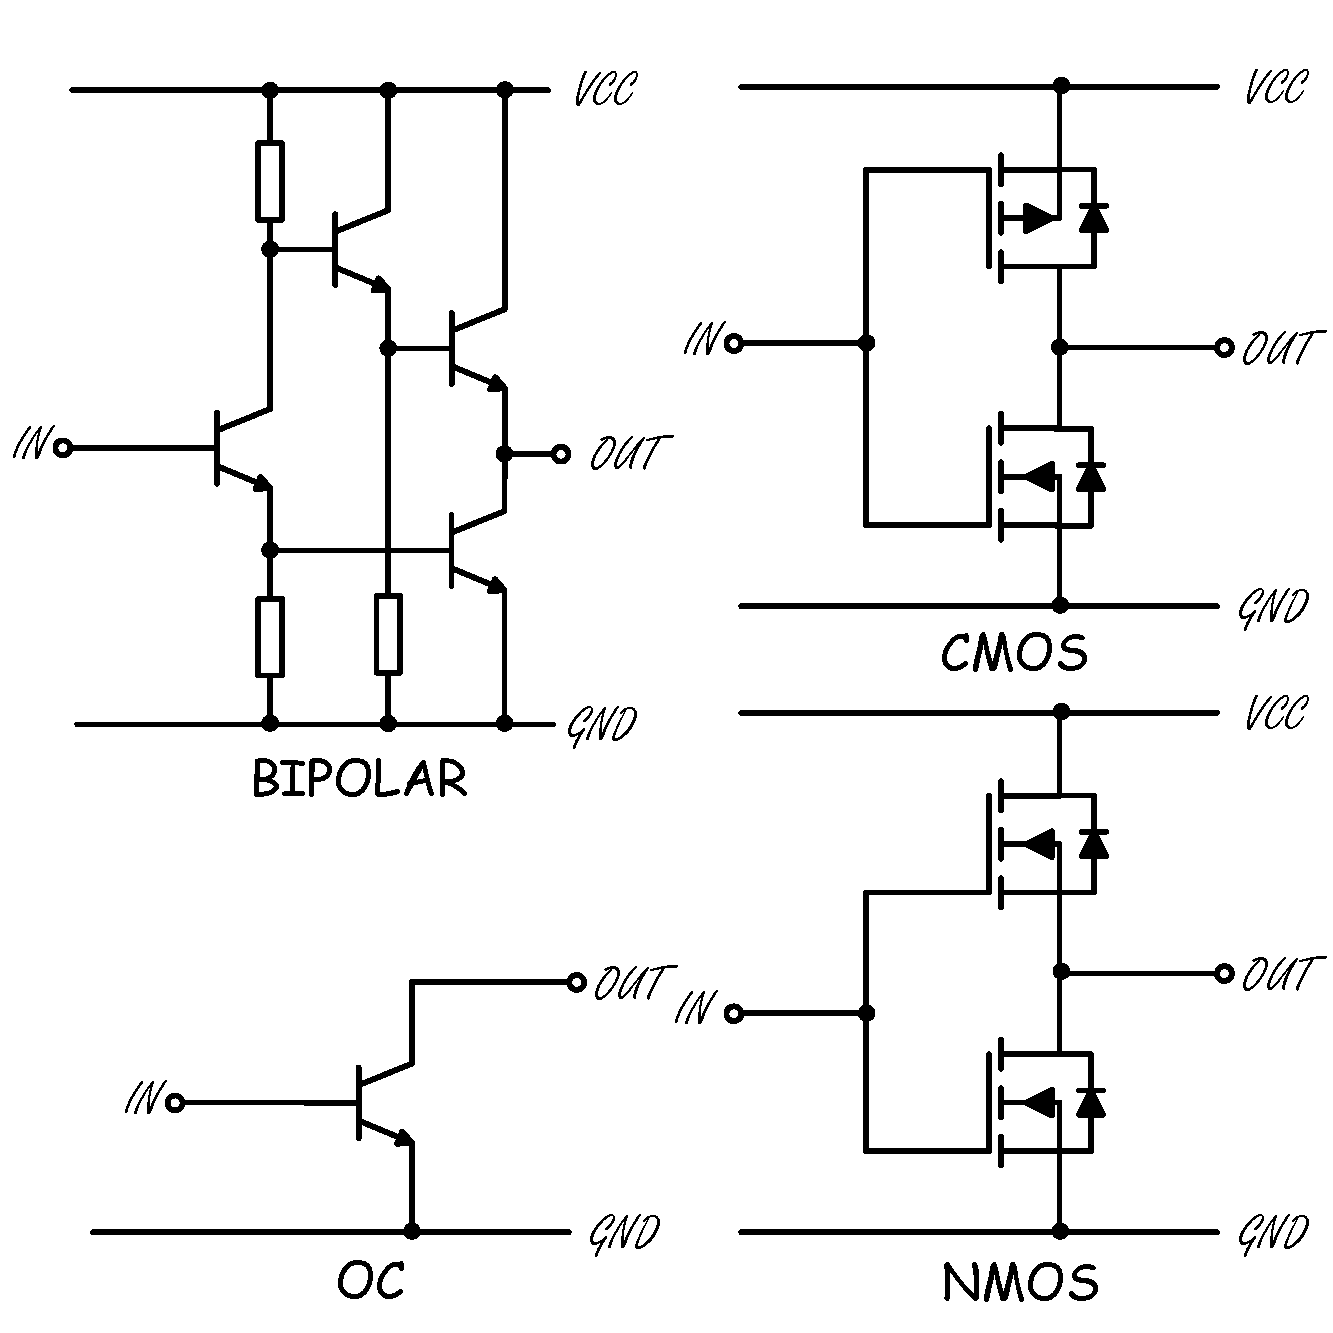
\includegraphics[width=0.7\linewidth]{digit_cir_output_common.pdf}
         \caption[Koncové stupně digitálních obvodů]
                 {Koncové stupně bipolárních, CMOS, NMOS obvodů a obvodů s otevřeným kolektorem 
                  \cite[p.~2]{AN240}}
         \label{ces:fig_digit_out_common}
    \end{figure}   
    
    % --------  Přizpůsobení: 3.3V -> 5V --------------------------- 
    \subsection{3.3V $\rightarrow$ 5V} %3.3V to 5V
      % The simplest and most desired way to connect a 3.3V output to a 5V input is by a direct
      % connection.  This can be done only if the following 2 requirements are met:
      Nejjednodušším a nejvíce žádoucím způsobem je přímé připojení 3.3V výstupu k 5V vstupu, což
      lze provést pouze v případě, že jsou splněny následující požadavky:
        \begin{itemize}\addtolength{\itemsep}{-0.5\baselineskip}
          \item $V_{OH}(3.3V)>V_{IH}(5V)$,
          \item $V_{OL}(3.3V)<V_{IL}(5V)$.
        \end{itemize}
      Hodnoty prahových napětí logické nuly a jedničky v předchozí tabulce \ref{CES:tab_threshold}
      dokládají, že v případě logiky \texttt{3.3V LVCMOS} a \texttt{5V TTL} je možné použít přímého
      připojení. 
      % An example of when this technique can  be used is interfacing a 3.3V LVCMOS output to a 5V
      % TTL input. From the values given in Table 4-1, it can clearly be  seen that both of these
      % requirements are met.

      % 3.3V LVCMOS VOH of 3.0 volts is greater than 5V TTL VIH of 2.0 volts and 3.3V LVCMOS VOL
      % of 0.5 volts is less than 5V TTL VIL of 0.8 volts.

      Pokud oba tyto požadavky nejsou splněny, je třeba použít na rozhraní obou logik
      přizpůsobovací obvody, popsané v následujících textu. 
      % When both of these requirements are  not met, some additional circuitry will be needed to
      % interface the two parts.

      \subsubsection{MOSFET Translator}
        \begin{figure}[ht!]
           \centering
           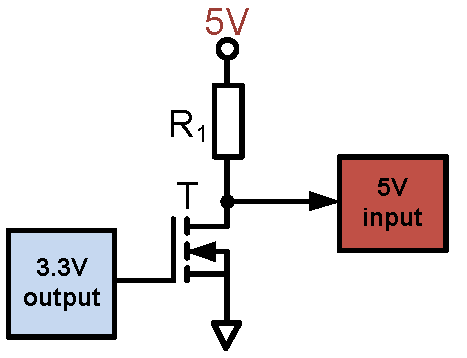
\includegraphics[scale=0.5]{level_shifting_MOSFET.pdf}
           \caption{3.3V $\rightarrow$ 5V: N-MOSFET}
           \label{CES:fig_shifting_MOSFET}
           \vspace*{-1\baselineskip}
        \end{figure}
        % In order to drive any 5V input that has a higher VIH than the VOH of a 3.3V CMOS part,
        % some additional circuitry is needed. A low-cost two component solution is shown in Figure
        % 6-1. When selecting the value for R1, there are two parameters that need to be considered;
        % the switching speed of the input and the current consumption through R1.
        Levné a jednoduché řešení problému vzájem\-ného přizpůsobení logických obvodů odliš\-ných
        napěťových tříd, pro které platí $V_{OH}(3.3V)<V_{IH}(5V)$ nabízí použití MOSFETu s
        prahovým napětím $$V_{GS_{th_{max}}}<V_{OH_{min}}.$$ Při výběru hodnoty $R_1$ je třeba vzít
        v úvahu:
        \begin{itemize}\addtolength{\itemsep}{-0.5\baselineskip}
          \item spínací rychlost vstupu,
          \item zvýšení spotřeby díky proudu přes rezistor $R_1$.
        \end{itemize}

        Při změně logické úrovně $'0'\rightarrow'1'$ na vstupu 5V logiky je nutné počítat se
        zpožděním, které je dáno časovou konstantu RC článku, tvořeného rezistorem $R_1$ a celkovou
        kapacitou na vstupu hradla. Důsledkem je tedy určitá minimální spínací perioda: 
        % When switching the input from a ‘0’ to a ‘1’, you will have to account for the time the
        % input takes to rise because of the RC time constant formed by R1, and the input
        % capacitance of the 5V input plus any stray capacitance on the board. The speed at which
        % you can switch the input is given by the following:
        $$T_{SW_{min}} = 3 \cdot R_1 \cdot C_{IN},$$ která je vyšší, čím nižší spotřeby se návrhář
        snaží dosáhnout ($R_1\uparrow$). Zpoždění při spínání $'1'\rightarrow'0'$ má příznivější
        hodnotu, neboť $R_{dsON}\ll R_1$.

        % Since the input and stray capacitance of the board are fixed, the only way to speed up
        % the switching of the input is to lower the resistance of R1. The trade-off of lowering
        % the resistance of R1 to get faster switching times is the increase in current draw when
        % the 5V input remains low. The switching to a ‘0’ will typically be much faster than
        % switching to a ‘1’ because the ON resistance of the N-channel MOSFET will be much smaller
        % than R1. Also, when selecting the N-channel FET, select a FET that has a lower VGS
        % threshold voltage than the VOH of 3.3V output.

      \subsubsection{Diodový Offset}
        Hodnoty vstupního prahového napětí \texttt{5V CMOS} a výstupní prahová napětí pro
        \texttt{3.3V LVTTL} a \texttt{LVCMOS} jsou uvedeny v tabulce \ref{CES:tab_diode_offset}
        % The inputs voltage thresholds for 5V CMOS and the output drive voltage for 3.3V LVTTL and
        % LVCMOS are listed in Table 7-1.
        \begin{table*}[t]
          \centering
          \begin{tabular}{|>{\columncolor{Tan}}l|c|c|c|}
            \hline
              \cellcolor{CornflowerBlue}                                   
                & \cellcolor{CornflowerBlue}\textbf{5V CMOS}       & 
              \cellcolor{CornflowerBlue} \textbf{3.3V LVTTL}               
                & \cellcolor{CornflowerBlue} \textbf{3.3V LVCMOS}  \\
              \multirow{-2}*{\cellcolor{CornflowerBlue}\texttt{Threshold}} 
                & \cellcolor{CornflowerBlue} IN 
                & \cellcolor{CornflowerBlue} OUT
                & \cellcolor{CornflowerBlue} OUT                   \\
            \hline\hline
               \texttt{High}                                               
                & $>3.5V$  & $>2.4V$ & $>3.0V$                     \\
               \texttt{Low}                                         
                & $<1.5V$  & $<0.4V$ & $<0.5V$                     \\
            \hline          
          \end{tabular}
          \caption{Přehled vstupní a výstupních prahový napětí různých logik, chceme-li ke vstupu
          \texttt{5V CMOS} připojit \texttt{3.3V LVTTL} nebo \texttt{3.3V LVCMOS.\cite{AN240}}}
          \label{CES:tab_diode_offset}
        \end{table*}

        \begin{figure}[ht!]
            \centering
            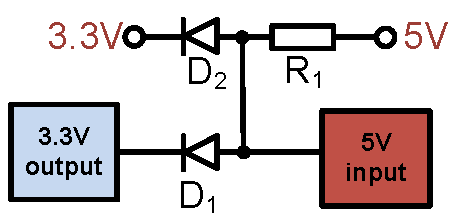
\includegraphics[scale=0.5]{level_shifting_diode_offset.pdf}
            \caption{3.3V $\rightarrow$ 5V: Diodový offset}
            \label{CES:fig_shifting_D_offset}
        \end{figure}

        Všimněme si, že obě prahová napětí vstupu \texttt{5V CMOS} logiky jsou o volt vyšší než u
        výstupu 3.3V logiky. Zapotřebí je tedy obvod, který zvyšuje vysokou a nízkou úroveň
        prahového napětí.
        % Note that both the high and low threshold input voltages for the 5V CMOS inputs are about
        % a volt higher than the 3.3V outputs. So, even if the output from the 3.3V system could be
        % offset, there would be little or no margin for noise or component tolerance. What is
        % needed is a circuit that offsets the outputs and increases the difference between the
        % high and low output voltages.

        Pokud bychom vytvořili posunutí o alespoň o 0.7V pro obě úrovně prahového napětí, dosáhli
        bychom vzájemného přizpůsobení. Obvod na obr. \ref{CES:fig_shifting_D_offset}, posuneme
        hodnotu nízké úrovně výstupního prahového napětí o úbytek v propustném směru diody $D_1$
        (typicky 0.7V), na 1.1V až 1.2V. Úroveň vysokého prahového napětí se nastavuje pomocí
        pull-up rezistoru a diody $D_2$ vázané na 3.3V napájení. Výstupní napětí je tedy také
        posunuto přibližně 0,7V nad 3,3V napájení, tj. na 4,0 až 4.1V, což je vysoko nad 3,5V
        prahem vstupu 5V CMOS logiky.

        % When output voltage specifications are determined, it is done assuming that the output is
        % driving a load between the output and ground for the high output, and a load between 3.3V
        % and the output for the low output. If the load for the high threshold is actually between
        % the output and 3.3V, then the output voltage is actually much higher as the load resistor
        % is the mechanism that is pulling the output up, instead of the output transistor.

        % If we create a diode offset circuit (see Figure 7-1), the output low voltage is increased
        % by the forward voltage of the diode D1, typically 0.7V, creating a low voltage at the 5V
        % CMOS input of 1.1V to 1.2V. This is well within the low threshold input voltage for the
        % 5V CMOS input. The output high voltage is set by the pull-up resistor and diode D2, tied
        % to the 3.3V supply. This puts the output high voltage at approximately 0.7V above the
        % 3.3V supply, or 4.0 to 4.1V, which is well above the 3.5V threshold for the 5V CMOS input
        \vskip2mm
        \begin{note}
          Aby obvod fungoval správně, musí být pull-up rezistor podstatně menší než vstupní odpor
          5V CMOS logiky, aby se zabránilo snížení výstupního napětí díky efektu vstupního
          odporového děliče a také musí být dostatečně velký, aby proud tekoucí do 3.3V napájení a
          výstupu hradla byl v mezích specifikace. 
          % For the circuit to work properly, the pull-up resistor must be significantly smaller
          % than the input resistance of the 5V CMOS input, to prevent a reduction in the output
          % voltage due to a resistor divider effect at the input. The pull-up resistor must also
          % be large enough to keep the output current loading on the 3.3V output within the
          % specification of the device.
        \end{note}

      \subsubsection{Komparátor}
        Základní funkce komparátoru je následující:        
        % The basic operation of the comparator is as follows:
        \begin{itemize}\addtolength{\itemsep}{-0.5\baselineskip}
          \item napětí na invertující (-) vstupu je větší než na neinvertujícím vstupu (+), výstup
                komparátoru se nastaví do nízké úrovně, 
                % When the voltage at the inverting (-) input is greater than that at the
                % non-inverting (+) input, the output of the comparator swings to Vss.
          \item je-li napětí na neinvertujícím vstupu (+) větší než na invertujícím vstupu (-),
                výstup komparátoru se nastaví do vysoké úrovně. %When the voltage at the
                % non-inverting (+) input is greater than that at the non-inverting (-)
                % input, the output of the comparator is in a high state.
        \end{itemize}

        \begin{figure}[ht!]
            \centering\vspace*{+1\baselineskip}
            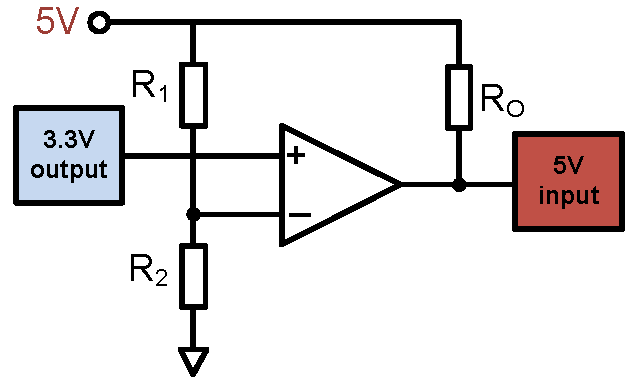
\includegraphics[scale=0.5]{level_shifting_COMP.pdf}
            \caption{3.3V $\rightarrow$ 5V: Komparátor; $R_1 = 1,8 k\Omega, R_2 = 1 k\Omega$}
            \label{CES:fig_shifting_COMP}           
        \end{figure}

        \textbf{Výpočet hodnoty odporu $R_1$ a $R_2$:}\newline
          Poměr R1 a R2 je závislý na napětí logické nuly a jedničky na výstupu hradla 3.3V logiky.
          Invertující vstup by měl být nastaven do poloviny mezi prahovými hladinami $V_{OL}$ a
          $V_{OH}$. Pro \texttt{LVCMOS} je toto napětí rovno $$1.75V = \frac{3V+0.5V}{2}.$$
          Budeme-li volit velikost $R_2$, pak hodnotu odporu $R_1$ snadno dopočítáme dle
          následující rovnice: $$R_1=R_2\left(\frac{5V}{1.75V}-1\right).$$ 
          % The ratio of R1  and R2  depends on the logic levels of the input signal. The inverting
          % input should be set to a voltage halfway between VOL and VOH for the 3.3V output. For
          % an LVCMOS output, this voltage is: $$1.75V = \frac{3V+0.5V}{2}.$$ Given that R1 and R2
          % are related by the logic levels:
          % $$R_1=R_2\left(\frac{5V}{1.75V}-1\right)$$ assuming a value of 1K for R2, R1 is 1.8K.

    % --------  Přizpůsobení: 5V -> 3.3V ---------------------------
    \subsection{5V $\rightarrow$ 3.3V} %5V to 3.3V
      \subsubsection{Přímé propojení}
        \begin{figure}[ht!]
            \centering
            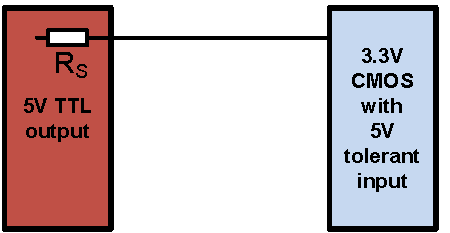
\includegraphics[scale=0.6]{direct_connect.pdf}
            \caption{5V $\rightarrow$ 3,3V: Přímé propojení}
            \label{CES:fig_dir_connect}
        \end{figure}

        Hradla napěťové třídy 5V mají výstupy s typickými prahovými hodnotami $V_{OH} = 4,7 V$,
        $V_{OL} = 0,4 V$ zatímco hradla 3.3V LVCMOS mají vstupy s prahovými hodnotami $V_{IH} =
        0,7\times V_{DD} $, $V_{IL} = 0,2\times V_{DD}$. Je-li tedy na 5V výstupu logická nula,
        bude také správně interpretována 3V vstupem, neboť platí $V_{OL} = 0,4 < V_{IL} = 0,8$. Ani
        v případě logické jedničky nevzniká žádný konflikt, neboť $V_{OH} = 4,7 > V_{IH} = 2,1$.
        Pokud je tedy 3V vstup 5V tolerantní, je možné přímé propojení, v opačném případě je třeba
        použít některou z následujících technik.
        % 5V outputs have a typical VOH of 4.7 volts and a VOL of 0.4 volts and a 3.3V LVCMOS input
        % will have a typical VIH of 0.7 x VDD and a VIL of 0.2 x VDD. When the 5V output is
        % driving low, there are no problems because the 0.4 volt output is less than in the input
        % threshold of 0.8 volts. When the 5V output is high, the VOH of 4.7 volts is greater than
        % 2.1 volt VIH, therefore, we can directly connect the 2 pins with no conflicts if the 3.3V
        % CMOS input is 5 volt tolerant. If the 3.3V CMOS input is not 5 volt tolerant, then there
        % will be an issue because the maximum volt specification of the input will be exceeded.

      \subsubsection{Diodový omezovač} %Diode Clamp
        Některé digitální obvody mají své vstupy chráněny vnitřními omezovacími diodami tzv.
        \texttt{diode clamp} (obr. \ref{CES:fig_int_clamp_D}). Proteče-li těmito diodami větší proud
        než udávají katalogové hodnoty, může dojít k poškození vstupu, nebo v lepším případě k
        efektu \texttt{latching-up}. Typický 5V výstup má kolem $10 \Omega$, proto chceme-li využít
        těchto diod, musíme přidat sériový odpor, jenž limituje velikost propustného proudu.
        Nepříjemným důsledkem je ovšem vzniklý RC článek se vstupní kapacitou hradla $C_L$, který
        snižuje rychlost. Není-li vstup takto chráněn je možné jej doplnit externí diodou dle obr.
        \ref{CES:fig_ext_clamp_D}.
        % Many manufacturers protect their I/O pins from exceeding the maximum allowable voltage
        % specification by using clamping diodes. These clamping diodes keep the pin from going
        % more than a diode drop below Vss and a diode drop above VDD. To use the clamping diode to
        % protect the input, you still need to look at the current through the clamping diode. The
        % current through the clamp diodes should be kept small (in the micro amp range). If the
        % current through the clamping diodes gets too large, then you risk the part latching up.
        % Since the source resistance of a 5V output is typically around 10 ohms, an additional
        % series resistor is still needed to limit the current through the clamping diode as shown
        % Figure 10-1. The consequence of using the series resistor is it will reduce the speed at
        % which we can switch the input because the RC time constant formed the capacitance of the
        % pin (CL).
       \begin{figure}[ht!]
         \centering
         \begin{tabular}{c}
           \subfloat[Vnitřními omezovací diody]{\label{CES:fig_int_clamp_D}
             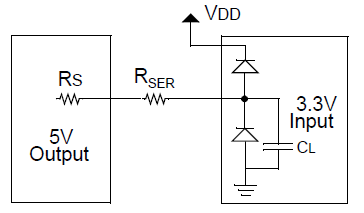
\includegraphics[width=0.3\textwidth]{CES_clamp_diodes_input.png}}        \\
           \subfloat[Externí omezovací dioda]{\label{CES:fig_ext_clamp_D}     
             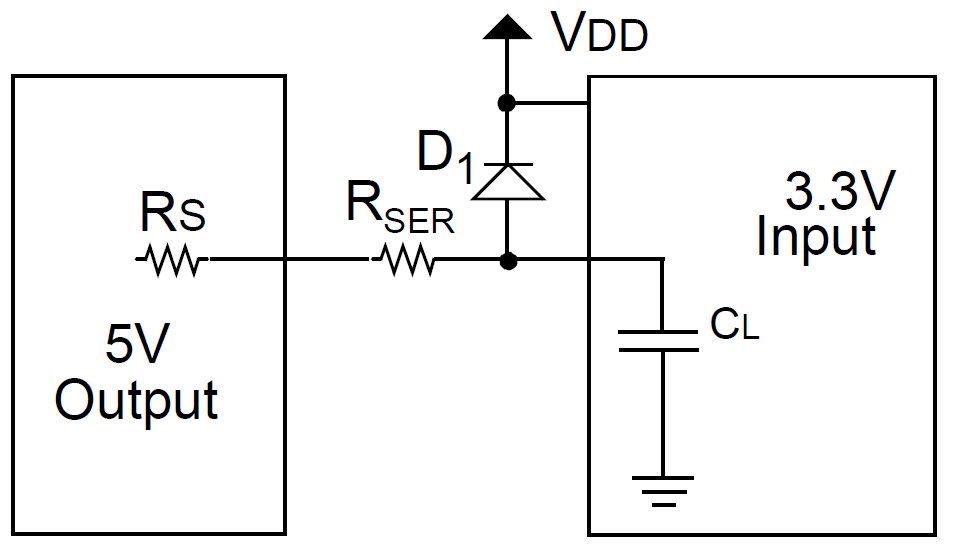
\includegraphics[width=0.3\textwidth]{CES_ext_clamp_diodes_input.png}}
         \end{tabular}  
         \caption{5V $\rightarrow$ 3,3V: Použití omezovacích diod pro ochranu vstupu integrovaného
                  obvodu}
         \label{CES:fig_clamp_diodes}
       \end{figure} 
        % One problem with using a diode clamp is that it injects current onto the 3.3V power
        % supply. In designs with a high current 5V outputs, and lightly loaded 3.3V power supply
        % rails, this injected current can float the 3.3V supply voltage above 3.3V. To prevent
        % this problem, a transistor can be substituted which routes the excess output drive
        % current to ground instead of the 3.3V supply.
          
        Dalším problémem je proud, injektovaný z 5V výstupu skrz omezovovací diodu do 3.3V
        napájení. Tento proud může způsobit zvýšení napájecího napětí 3.3V obvodů, což může vést k
        jejich zničení. Proto lze s výhodou použít PNP tranzistor zapojený dle obr.
        \ref{CES:fig_bjt_clamp}.
        
        \begin{figure}[ht!]
          \centering
          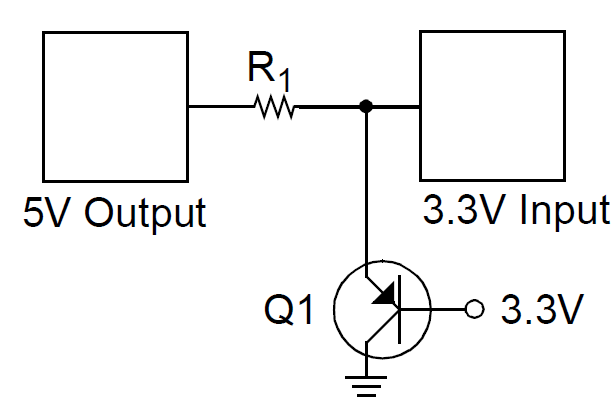
\includegraphics[scale=0.5]{CES_ext_clamp_bjt_input.png}
          \caption{5V $\rightarrow$ 3,3V: Active clamp - Přechod báze-emitor funguje jako omezovací
                   dioda, ovšem s tím rozdílem, že jen malé procento celkového proudu z 5V výstupu
                   teče do 3.3V napájení. Převážná část teče kolektorem do země. Poměr bázového a
                   kolektorového proudu je určen proudovým zesílením tranzistoru, které je typicky
                  10 až 400}
          \label{CES:fig_bjt_clamp}
        \end{figure}              
       
      \subsubsection{Napěťový dělič} %Resistor divider
        A simple resistor divider can be used to reduce the output of a 5V device to levels
        appropriate for a 3.3V device input. An equivalent circuit of this interface is shown in
        Figure \ref{CES:fig_res_divider}.
        \begin{figure}[ht!]
          \centering
          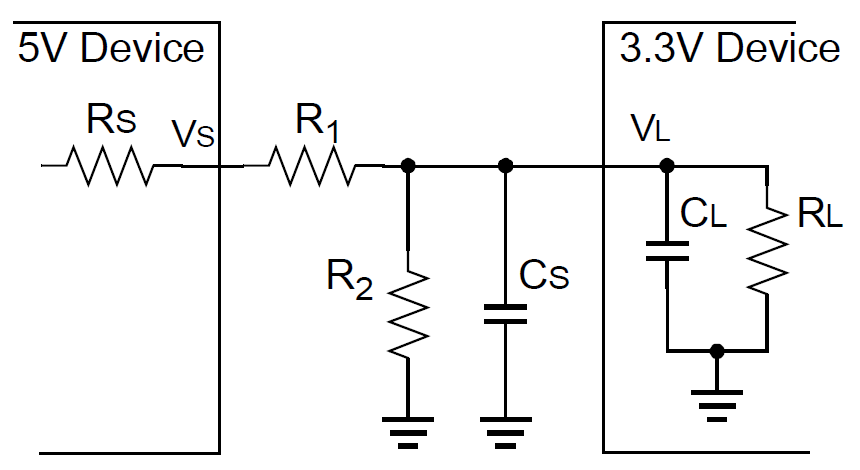
\includegraphics[scale=0.4]{CES_ext_res_divider.png}
          \caption{5V $\rightarrow$ 3,3V: napěťový děliš}
          \label{CES:fig_res_divider}
        \end{figure}
        Typically, the source resistance, $R_S$, is very small (less than 10 ohms) so its affect on
        $R_1$ will be negligible provided that $R_1$ is chosen to be much larger than $R_S$. At the
        receive end, the load resistance, $R_L$, is very large (greater than 500 k ohms) so its
        affect on $R_2$ will be negligible provided that $R_2$ is chosen to be much less than
        $R_L$.
        
        There is a trade-off between power dissipation and transition times. To keep the power
        requirements of the interface circuit at a minimum, the series resistance of $R_1$ and
        $R_2$ should be as large as possible. However, the load capacitance, which is the
        combination of the stray capacitance, $C_S$, and the 3.3V device input capacitance, $C_L$,
        can adversely affect the rise and fall times of the input signal. Rise and fall times can
        be unacceptably long if $R_1$ and $R_2$ are too large.
        
        Neglecting the affects of $R_S$ and $R_L$, the formula for determining the values for $R_1$
        and $R_2$ is given by Equation \ref{CES:eq_res_divider}.
        \begin{align}\label{CES:eq_res_divider}
          \frac{V_S}{R_1+R_2} &= \frac{V_L}{R_2}           \nonumber \\
                          R_1 &= \frac{(V_S-V_L)}{V_L}R_2  \nonumber \\
                          R_1 &= 0,515\cdot R_2
        \end{align}      
        The formula for determining the rise and fall times is given in Equation
        \ref{CES:eq_res_divider_time}. For circuit analysis, the Thevenin equivalent is used to
        determine the applied voltage, $V_A$, and the series resistance, $R$.
        The Thevenin equivalent is defined as the open circuit voltage divided by the short circuit
        current. The Thevenin equivalent, $R$, is determined to be $0.66\cdot R_1$ and the Thevenin
        equivalent, $V_A$, is determined to be $0.66\cdot V_S$ for the circuit shown in  Figure
        \ref{CES:fig_res_divider} according to the limitations imposed by Equation
        \ref{CES:eq_res_divider_time}.
        \begin{equation}\label{CES:eq_res_divider_time}
          t = - R\cdot C \cdot \ln\left(\frac{V_F-V_A}{V_I-V_A}\right)
        \end{equation}  
        kde $t$ = Rise or Fall time, $R = 0.66\cdot R_1$, $C = C_S+C_L$, $V_I$ = Initial voltage on
        $C$ ($V_L$), $V_F$ = Final voltage on $C$ ($V_L$), $V_A$ = Applied voltage ($0.66\cdot V_S$). 
        \begin{example} As an example, suppose the following conditions exist:
          \begin{itemize}\addtolength{\itemsep}{-0.5\baselineskip}
            \item Stray capacitance = 30 pF,
            \item Load capacitance = 5 pF,
            \item Maximum rise time from 0.3V to 3V ≤ 1 μS
            \item Applied source voltage Vs = 5V
          \end{itemize}
          Solve Equation \ref{CES:eq_res_divider_time} for $R$:  
          \begin{equation*}
            R = - \dfrac{t}{C\cdot\ln\dfrac{V_F-V_A}{V_I-V_A}}
          \end{equation*}   
          Substitute values:
          \begin{equation*}
            R = - \dfrac{10\cdot10^{-7}}{35\cdot10^{-12}\cdot
                  \ln\dfrac{3-0.66\cdot5}{0.3-0.66\cdot5}}
          \end{equation*}               
          Thevenin equivalent maximum R: $$R = 12408$$
          Solve for maximum $R_1$ and $R_2$:
          \begin{alignat}{3}
            & R_1 &&= 0.66\cdot R  \qquad &&R_2 = \frac{R_1}{0.515}  \\
            & R_1 &&= 8190         \qquad &&R_2 = 15902 
          \end{alignat}          
        \end{example} 
                   
      \subsubsection{Level translator} %Level translator
        While level translation can be done discretely, it is often preferred to use an integrated
        solution. Level translators are available in a wide range of capabilities. There are
        unidirectional and bidirectional configurations, different voltage translations and
        different speeds, all giving the user the ability to select the best solution. 
        \begin{figure}[ht!]
          \centering
          \begin{tabular}{c}
            \subfloat[SPI sběrnice]{\label{CES:fig_level_translator1}
              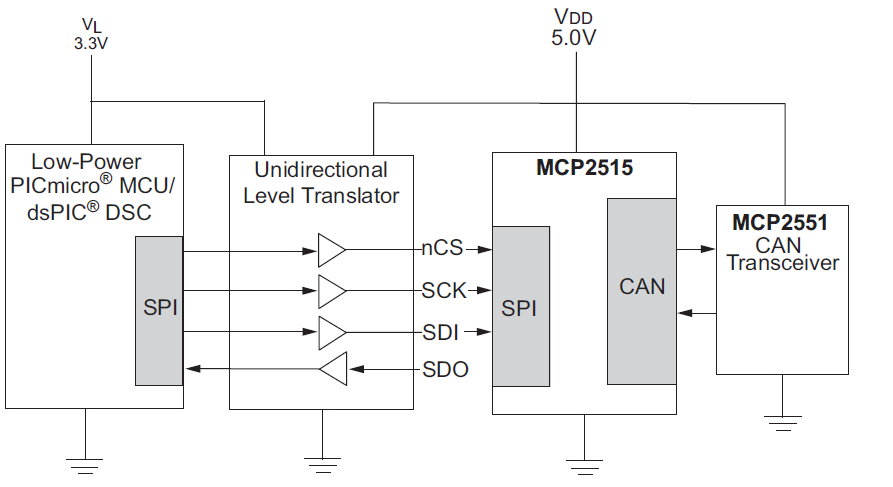
\includegraphics[width=0.9\linewidth]{CES_ext_level_translator1.png}}           \\
            \subfloat[I2C sběrnice]{\label{CES:fig_level_translator2}
              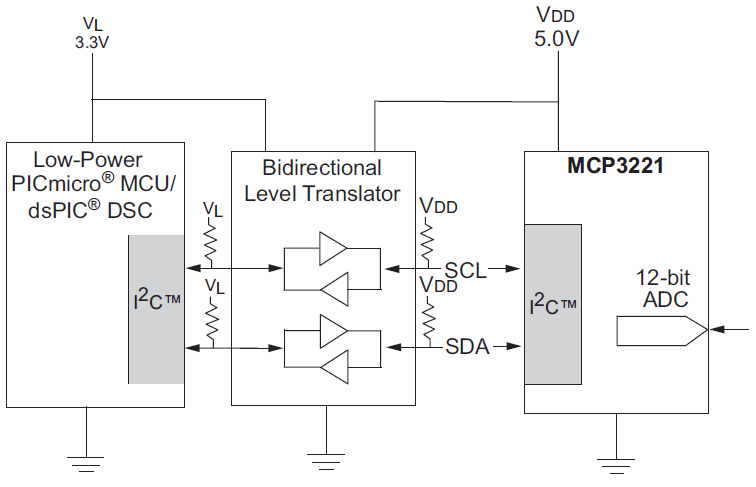
\includegraphics[width=0.9\linewidth]{CES_ext_level_translator2.png}}
          \end{tabular}  
          \caption{5V $\rightarrow$ 3,3V: Board-level communication between devices (e.g., MCU to
                   peripheral) is most often done by either SPI or I2C. For SPI, it may be
                   appropriate to use a unidirectional level translator and for I2C, it is necessary
                   to use a bidirectional solution.}
          \label{CES:fig_level_translator}
        \end{figure}           
      
} % tikzset
%---------------------------------------------------------------------------------------------------
\printbibliography[title={Seznam literatury}, heading=subbibliography]
\addcontentsline{toc}{section}{Seznam literatury}